%!TEX root = IntensionalSemantics.tex
\chapter{Beginnings}\label{cha:beginnings_of_intensional_semantics} % (fold)

\epigraph{Language is the main instrument of man's refusal to accept
  the world as it is.}{George Steiner, \emph{After Babel}, p. 228}

\chapterprecishere{We introduce the idea of extension vs. intension
  and its main use: taking us from the actual here and now to past,
  future, possible, counterfactual situations. We develop a
  compositional framework for intensional semantics.}

\minitoc

\section{Displacement} \label{sec:displacement}

\citet{hockett:origin:60}\sidepar{\fullcite{hockett:origin:60}} in
a famous article (and a follow-up, \citet{hockett:design:68})
presented a list of \term{design features of human language}. This
list continues to play a role in current discussions of animal
communication. One of the design features is \term{displacement}.
Human language is not restricted to discourse about the \emph{actual
  here and now}.\footnote{\citet[226]{steiner:1998:babel} writes:
  ``Hypotheticals, `imaginaries', conditionals, the syntax of
  counter-factuality and contingency may well be the generative
  centres of human speech''.}

How does natural language untie us from the actual here and now? One
degree of freedom is given by the ability to name entities and refer
to them even if they are not where we are when we speak:

\ex. Thomas is in Hamburg.

This kind of displacement is not something we will explore here. We'll
take it for granted.

Consider a sentence with no names of absent entities in it:

\ex. It is snowing (in Cambridge).

On its own, \Last makes a claim about what is happening right now here
in Cambridge. But there are devices at our disposal that can be added
to \Last, resulting in claims about snow in displaced situations.
Displacement can occur in the \term{temporal} dimension and/or in what
might be called the \term{modal}\sidepar{The terms \term{modal}
  and \term{modality} descend from the Latin \expression{modus},
  ``way'', and are ancient terms pertaining to the way a proposition
  holds, necessarily, contingently, etc.} dimension. Here's an example
of temporal displacement:

\ex. At noon yesterday, it was snowing in Cambridge.

This sentence makes a claim not about snow now but about snow at noon
yesterday, a different time from now.

Here's an example of modal displacement:

\ex. If the storm system hadn't been deflected by the jet stream, it
would have been snowing in Cambridge.

This sentence makes a claim not about snow in the actual world but
about snow in the world as it would have been if the storm system
hadn't been deflected by the jet stream, a world distinct from the
actual one (where the system did not hit us), a merely \term{possible
  world}.

Natural %
\sidepar{See \citet{kratzer:1981:notional,kratzer:1991:modality} for
  more examples of modal constructions.}%
language abounds in modal constructions. \Last is a so-called
\term{counterfactual conditional}. Here are some other examples:

\ex. \term{Modal Auxiliaries}\\
It may be snowing in Cambridge.

\ex. \term{Modal Adverbs}\\
Possibly, it will snow in Cambridge tomorrow.

\ex. \term{Propositional Attitudes}\\
Jens believes that it is snowing in Cambridge.

\ex. \term{Habituals}\\
Jane smokes.

\ex. \term{Generics}\\
Bears like honey.

% The plan for this course is as follows. In Part 1, we explore modality
% and associated topics. In Part 2, we explore temporal matters.

In this chapter, we will put in place the basic framework of
\term{intensional semantics}, the kind of semantics that models
displacement of the point of evaluation in temporal and modal
dimensions. To do this, we will start with one rather special example
of modal displacement:

\ex.\label{sherlock} In the world of Sherlock Holmes, a detective
lives at 221B Baker Street.

\Last\marginpar{\raggedleft
\includegraphics[width=1in]{sherlock-holmes-147255.png}}\marginnote{
\url{https://en.wikipedia.org/wiki/Sherlock_Holmes}} doesn't claim that a
detective lives at 221B Baker Street in the actual world (presumably a
false claim), but that in the world as it is described in the Sherlock
Holmes stories of Sir Arthur Conan Doyle, a detective lives at 221B
Baker Street (a true claim, of course). We choose this example rather
than one of the more run-of-the-mill displacement constructions
because we want to focus on conceptual and technical matters before we
do serious empirical work.

The questions we want to answer are: How does natural language achieve
this feat of modal displacement? How do we manage to make claims about
other possible worlds? And why would we want to?

To make displacement possible and compositionally tractable, we need
meanings of natural language expressions, and of sentences in
particular, to be displaceable in the first place. They need to be
``portable'', so to speak, able to make claims about more than just
the actual here and now. And need we need other natural language
expressions that take that portable meaning and apply it to some
situation other than the actual here and now. That is what
intensionality is all about.

The basic idea of the account we'll develop is this:

\begin{itemize}
\item expressions are assigned their semantic values relative to a
  possible world;
\item in particular, sentences have truth-values in possible worlds;
\item in the absence of modal displacement, we evaluate sentences with
  respect to the ``actual'' world, the world in which we are speaking;
\item modal displacement changes the world of evaluation;
\item displacement is effected by special operators, whose semantics
  is our primary concern here.
\end{itemize}
%
A terminological note: we will call the sister of the intensional
operator its \term{prejacent}, a useful term introduced by our
medieval colleagues.

\clearpage
\section{An Intensional Semantics in 10 Easy Steps} \label{sec:an-intens-semant}

\subsection{Laying the Foundations} \label{sec:laying-foundations}

\subsubsection{Step 1: Possible Worlds.} \label{sec:world-parameter}

Our first step is to introduce possible worlds. This is not the place
to discuss the metaphysics of possible worlds in any depth. Instead,
we will just start working with them and see what they can do for us.
Basically, a possible world is a way that things might have been. In
the actual world, there are two coffee mugs on my desk, but there
could have been more or less. So, there is a possible world \dash
albeit a rather bizarre one \dash where there are 17 coffee mugs on my
desk. We join Heim \amp\ Kratzer in adducing this quote from
\citet[1f.]{lewis:plurality:1986}\marginpar{\centering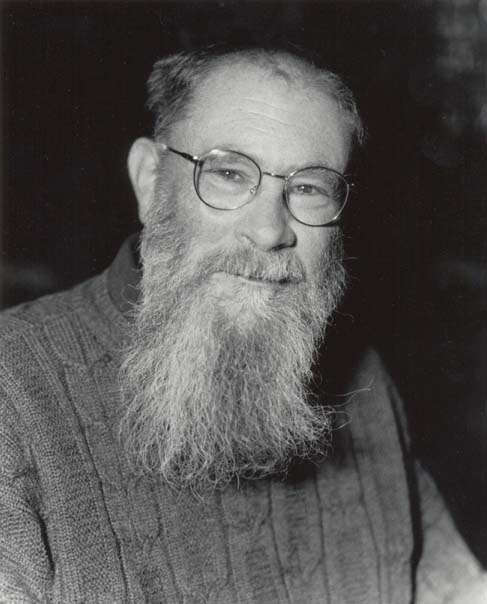
\includegraphics[height=1in]{lewis.jpg}\\
  {\tiny
    \href{http://en.wikipedia.org/wiki/David_Lewis_(philosopher)}{David
      Lewis}}}:

\begin{quote}
  The world we live in is a very inclusive thing. Every stick and
  every stone you have ever seen is part of it. And so are you and I.
  And so are the planet Earth, the solar system, the entire Milky Way,
  the remote galaxies we see through telescopes, and (if there are
  such things) all the bits of empty space between the stars and
  galaxies. There is nothing so far away from us as not to be part of
  our world. Anything at any distance at all is to be included.
  Likewise the world is inclusive in time. No long-gone ancient
  Romans, no long-gone pterodactyls, no long-gone primordial clouds of
  plasma are too far in the past, nor are the dead dark stars too far
  in the future, to be part of the same world. \dots
	
  \medskip
	
  The way things are, at its most inclusive, means the way the entire
  world is. But things might have been different, in ever so many
  ways. This book of mine might have been finished on schedule. Or,
  had I not been such a commonsensical chap, I might be defending not
  only a plurality of possible worlds, but also a plurality of
  impossible worlds, whereof you speak truly by contradicting
  yourself. Or I might not have existed at all \dash neither myself,
  nor any counterparts of me. Or there might never have been any
  people. Or the physical constants might have had somewhat different
  values, incompatible with the emergence of life. Or there might have
  been altogether different laws of nature; and instead of electrons
  and quarks, there might have been alien particles, without charge or
  mass or spin but with alien physical properties that nothing in this
  world shares. There are ever so many ways that a world might be: and
  one of these many ways is the way that this world is.
\end{quote}
%
Previously, our ``metaphysical inventory'' included a domain of
entities and a set of two truth-values and increasingly complex
functions between entities, truth-values, and functions thereof. Now,
we will add possible worlds to the inventory. Let's assume we are
given a set $W$, the set of all possible worlds, which is a vast space
since there are so many ways that things might have been different
from the way they are. Each world has as among its parts entities like
you and me and these coffee mugs. Some of them may not exist in other
possible worlds. So, strictly speaking each possible worlds has its
own, possibly distinctive, domain of entities. What we will use in our
system, however, will be the grand union of all these world-specific
domains of entities. We will use $D$ to stand for the set of all
possible individuals.

Among the many possible worlds that there are \dash according to
Lewis, there is a veritable plenitude of them \dash is the world as it
is described in the Sherlock Holmes stories by Sir Arthur Conan Doyle.
In that world, there is a famous detective Sherlock Holmes, who lives
at 221B Baker Street in London and has a trusted sidekick named Dr.
Watson. Our sentence \expression{In the world of Sherlock Holmes, a
  detective lives at 221B Baker Street} displaces the claim that a
famous detective lives at 221B Baker Street from the actual world to
the world as described in the Sherlock Holmes stories. In other words,
the following holds:\footnote{We will see in Section
  \ref{sec:why-talk-about} that this is not quite right. It'll do for
  now.}

\ex. The sentence \expression{In the world of Sherlock Holmes, a
  detective lives at 221B Baker Street} is true in a world w iff the
sentence \expression{a detective lives at 221B Baker Street} is true
in the world as it is described in the Sherlock Holmes stories.

What this suggests is that we need to make space in our system for
having devices that control in what world a claim is evaluated. This
is what we will do now.

\subsubsection{Step 2: The Evaluation World Parameter.} \label{sec:eval-world-param}

Recall from H\amp K that we were working with a semantic
interpretation function that was relativized to an assignment function
$g$, which was needed to take care of pronouns, traces, variables,
etc. From now on, we will relativize the semantic values in our system
to possible worlds as well. What this means is that from now on, our
interpretation function will have two superscripts: a world $w$ and an
assignment $g$: $\sv{\mbox{\textperiodcentered}}^{w,g}$.

So, the prejacent embedded in \ref{sherlock} will have its
truth-conditions described as follows:\footnote{Recall from H\amp\ K,
  pp.22f, that what's inside the interpretation brackets is a mention
  of an object language expression. They make this clear by
  bold-facing all object language expressions inside interpretation
  brackets. In these notes, we will follow common practice in the
  field and not use a special typographic distinction, but let it be
  understood that what is interpreted are object language
  expressions.}

\ex. $\sv{\mbox{a famous detective lives at 221B Baker Street}}^{w,g} = 1$\\
iff a famous detective lives at 221B Baker Street in world $w$.

It is customary to refer to the world for which we are calculating the
extension of a given expression as the \term{evaluation world}. In the
absence of any shifting devices, we would normally evaluate a sentence
in the actual world. But then there are shifting devices such as our
\expression{in the world of Sherlock Holmes}. We will soon see how
they work. But first some more pedestrian steps: adding lexical
entries and composition principles that are formulated relative to a
possible world. This will allow us to derive the truth-conditions as
stated in \Last in a compositional manner.

\subsubsection{Step 3: Lexical Entries.} \label{sec:lexical-entries}

Among our lexical items, we can distinguish between items which have a
\term{world-dependent} semantic value and those that are
world-independent. Predicates are typically world-dependent. Here are
some sample entries.

\ex. For any $w \in W$ and any assignment function $g$: \a.
$\sv{\mbox{famous}}^{w,g} = \lambda x \in D.\ x \mbox{ is famous in }
w$.%
\footnote{Of course, ``$\lambda x \in D.\ \dots$'' is short for
  ``$\lambda x\co x \in D.\ \dots$''. Get used to semanticists
  condensing their notation whenever convenient! A further step of
  condensation is taken below: ``$\lambda x\co x \in D_e.\ \dots$''
  becomes ``$\lambda x_e.\ \dots$''.}$^{,}$%
\footnote{Always make sure that you actually understand what the
  notation means. Here, for example, we are saying that the semantic
  value of the word \emph{famous} with respect to a given possible
  world $w$ and a variable assignment $g$ is that function that is
  defined for an argument $x$ only if $x$ is a member of the domain of
  individuals and that, if it is defined, yields the truth-value 1 if
  and only if $x$ is famous in $w$.} \b.
$\sv{\mbox{detective}}^{w,g} = \lambda x \in D.\ x \mbox{ is a
  detective in } w$.
\b.
$\sv{\mbox{lives-at}}^{w,g} = \lambda x \in D.\ \lambda y \in D.\ y
\mbox{ lives-at } x \mbox{ in } w $.

The set of detectives will obviously differ from world to world, and
so will the set of famous individuals and the set of pairs where the
first element lives at the second element.

Other items have semantic values which do not differ from world to
world. The most important such items are certain ``logical''
expressions, such as truth-functional connectives and
determiners:

\ex. \a.
$\sv{\mbox{and}}^{w,g} = \lambda u \in D_t.\ \lambda v \in D_t.\ u=v=1
$.
\b.
$\sv{\mbox{the}}^{w,g} = \lambda f \in D_{\angles{e,t}}\co \exists !
x[f(x) = 1]. \mbox{ the } y \mbox{ such that } f(y) = 1$.
\b.
$\sv{\mbox{every}}^{w,g} = \lambda f_{\angles{e,t}}.\ \lambda
h_{\angles{e,t}}.\ \forall x_e\co f(x) = 1 \rightarrow h(x) = 1 $.
\sidepar{Note the ruthless condensation of the notation in (c) and
  (d): variables are subscripted with the type of the domain that
  their values are constrained to come from.} \c.
$\sv{\mbox{a/some}}^{w,g} = \lambda f_{\angles{e,t}}.\ \lambda
h_{\angles{e,t}}.\ \exists x_e\co f(x) = 1\ \&\ h(x) = 1 $.

Note that there is no occurrence of $w$ on the right-hand side of the
entries in \Last. That's the tell-tale sign of the world-independence
of the semantics of these items.

We will also assume that proper names have world-independent semantic
values, that is, they refer to the same individual in any possible
world.

\ex. \a. $\sv{\mbox{Noam Chomsky}}^{w,g}$ = Noam Chomsky. 
\b. $\sv{\mbox{Sherlock Holmes}}^{w,g}$ = Sherlock Holmes. 
\c. $\sv{\mbox{221B Baker Street}}^{w,g}$ = 221B Baker Street.

\subsubsection{Step 4: Composition Principles.} \label{sec:comp-princ}

The old rules of Functional Application, Predicate Modification, and
$\lambda$-Abstraction can be retained almost intact. We just need to
modify them by adding world-superscripts to the interpretation
function. For example:

\ex. \term{Functional Application (FA)}\\
If $\alpha$ is a branching node and $\{\beta, \gamma\}$ the set of its
daughters, then, for any world $w$ and assignment $g$: if
$\sv{\beta}^{w,g}$ is a function whose domain contains
$\sv{\gamma}^{w,g}$, then
$\sv{\alpha}^{w,g} = \sv{\beta}^{w,g} (\sv{\gamma}^{w,g})$.

The rule simply passes the world parameter down.

\subsubsection{Step 5: Truth.} \label{sec:truth}

Lastly, we will want to connect our semantic system to the notion of
the \term{truth of an utterance}. We first adopt the ``Appropriateness
Condition'' from Heim \amp\ Kratzer (p.243):

\ex. \extitle{Appropriateness Condition}\\
A context $c$ is \emph{appropriate} for an LF $\phi$ only if $c$
determines a variable assignment $g_c$ whose domain includes every
index which has a free occurrence in $\phi$.

We then intensionalize Heim \amp\ Kratzer's definition of truth and
falsity of utterances:

\ex. \extitle{Truth and Falsity Conditions for Utterances}\\
An utterance of a sentence $\phi$ in a context $c$ in a possible world $w$ is \emph{true} iff $\sv{\phi}^{w,g_c} = 1$ and \emph{false} if $\sv{\phi}^{w,g_c} = 0$.

\begin{exercise}
  Compute under what conditions an utterance in possible world $w_7$
  (which may or may not be the one we are all living in) of the
  sentence \expression{a famous detective lives at 221B Baker Street}
  is true. [Since this is the first exercise of the semester, please
  do this in excrutiating detail, not skipping any steps.] \eex
\end{exercise}

\subsection{Intensional Operators} \label{sec:intens-oper}

So far we have merely ``redecorated'' our old system inherited from
last semester. We have introduced possible worlds into our inventory,
our lexical entries and our old composition principles. But with the
tools we have now, all we can do so far is to keep track of the world
in which we evaluate the semantic value of an expression, complex or
lexical. We will get real mileage once we introduce \term{intensional
  operators} which are capable of shifting the world parameter. We
mentioned that there are a number of devices for modal displacement.
As advertised, for now, we will just focus on a very particular one:
the expression \expression{in the world of Sherlock Holmes}. We will
assume, as seems reasonable, that this expression is a
sentence-modifier both syntactically and semantically.

\subsubsection{Step 6: A Syncategorematic Entry.} \label{sec:sync-entry}

We begin with a heuristic step. We want to derive something like the
following truth-conditions for our sentence:

\ex. $\sv{\mbox{in the world of Sherlock Holmes,}\\
\mbox{a famous detective lives at 221B Baker Street}}^{w,g} = 1$\\
iff the world $w'$ as it is described in the Sherlock Holmes stories is such that there exists a famous detective in $w'$ who lives at 221B Baker Street in $w'$.

We would get this if in general we had this rule for \expression{in
  the world of Sherlock Holmes}:

\ex. For any sentence $\phi$, any world $w$, and any assignment $g$:\\
$\sv{\mbox{in the world of Sherlock Holmes }\phi}^{w,g} = 1$\\
iff the world $w'$ as it is described in the Sherlock Holmes stories is such that $\sv{\phi}^{w',g} = 1$.

This is a so-called \term{syncategorematic} treatment of the meaning
of this expression. Instead of giving an explicit semantic value to
the expression, we specify what effect it has on the meaning of a
complex expression that contains it. In \Last, we do not compute the
meaning for \expression{in the world of Sherlock Holmes, $\phi$} from
the combination of the meanings of its parts, since \expression{in the
  world of Sherlock Holmes} is not given a separate meaning, but in
effect triggers a special composition principle. This %
\sidepar{The diamond $\diamondsuit$ symbol for possibility is due to
  C.I. Lewis, first introduced in
  \citet{lewis-langford:1932:symbolic}, but he made no use of a symbol
  for the dual combination $\neg\diamondsuit\neg$. The dual symbol
  $\square$ was later devised by F.B. Fitch and first appeared in
  print in 1946 in a paper by his doctoral student
  \citet{barcan:1946:calculus}. See footnote 425 of
  \citet{hughes-cresswell:1968:introduction}. Another notation one
  finds is $L$ for necessity and $M$ for possibility, the latter from
  the German \expression{möglich} `possible'.}%
format is very common in modal logic systems, which usually give a
syncategorematic semantics for the two modal operators (the necessity
operator $\square$ and the possibility operator $\diamondsuit$). When
one only has a few closed class expressions to deal with that may
shift the world parameter, employing syncategorematic entries is a
reasonable strategy. But we are facing a multitude of displacement
devices. So, we will need to make our system more modular.

So, we want to give \expression{in the world of Sherlock Holmes} its
own meaning and combine that meaning with that of its prejacent by a
general composition principle. The Fregean slogan we adopted says that
all composition is function application (modulo the need for
$\lambda$-abstraction and the possible need for predicate
modification).\footnote{See Heim \amp\ Kratzer, Section 4.3, pp.
  63--72 for a reminder about the status of predicate modification.}
So, what we will want to do is to make \LLast be the result of
functional application. But we can immediately see that it cannot be
the result of our usual rule of functional application, since that
would feed to \expression{in the world of Sherlock Holmes} the
semantic value of \expression{a famous detective lives in 221B Baker
  Street} in $w$, which would be a particular truth-value, $1$ if a
famous detective lives at 221B Baker Street in $w$ and $0$ if there
doesn't. And whatever the semantics of \expression{in the world of
  Sherlock Holmes} is, it is certainly \emph{not} a truth-functional
operator.

So, we need to feed something else to \expression{in the world of
  Sherlock Holmes}. At the same time, we want the operator to be able
to shift the evaluation world of its prejacent. Can we do this?

\begin{exercise}
    How would you show that \expression{in the world of Sherlock
      Holmes} is not a truth-functional operator? \eex
\end{exercise}

\subsubsection{Step 7: Intensions.} \label{sec:intensions}

We will define a richer notion of semantic value, the \term{intension}
of an expression. This will be a function from possible worlds to the
extension of the expression in that world. The intension of a sentence
can be applied to any world and give the truth-value of the sentence
in that world. Intensional operators take the intension of their
prejacent as their argument, that is we will feed the intension of the
embedded sentence to the shifting operator. The operator will use that
intension and apply it to the world it wants the evaluation to happen
in. Voilà.

Now %
\sidepar{As before in H\amp\ K, we make no claim that the semantic
  values that are attributed to expressions in our framework fully
  capture what is informally meant by ``meaning''. But certainly,
  intensions come close to ``meaning'' than extensions.}%
let's spell that account out. Our system actually provides us with two
kinds of meanings. For any expression $\alpha$, we have
$\sv{\alpha}^{w,g}$, the semantic value of $\alpha$ in $w$, also known
as the \term{extension} of $\alpha$ in $w$. But we can also calculate
$\lambda w. \sv{\alpha}^{w,g}$, the function that assigns to any world
$w$ the extension of $\alpha$ in that world. This is usually called
the \term{intension} of $\alpha$. We will sometimes use an
abbreviatory notation\footnote{The notation with the subscripted
  cent-sign comes from Montague Grammar. See e.g.
  \citet[147]{dowty-wall-peters:1981:intro}.} for the intension of
$\alpha$:

\ex. $\svcent{\alpha}^g := \lambda w. \sv{\alpha}^{w,g}$.

It should be immediately obvious that since the definition of
intension abstracts over the evaluation world, intensions are not
world-dependent.\footnote{Since intensions are by definition not
  dependent on the choice of a particular world, it makes no sense to
  put a world-superscript on the intension-brackets. So don't ever
  write ``$\svcent{\dots}^{w,g}$''; we'll treat that as undefined
  nonsense.}\footnote{The definition here is simplified, in that it
  glosses over the fact that some expressions, in particular those
  that contain \term{presupposition triggers}, may fail to have an
  extension in certain worlds. In such a case, the intension has no
  extension to map such a world to. Therefore, the intension will have
  to be a partial function. So, the official, more ``pedantic'',
  definition will have to be as follows:
  $\sv{\alpha}_{\tiny \mbox{\textcent}}^g := \lambda w\co \alpha \in
  \mbox{dom}(\sv{\null}^{w,g}). \sv{\alpha}^{w,g}$.}

Note that strictly speaking, it now makes no sense anymore to speak of
``\emph{the} semantic value'' of an expression $\alpha$. What we have
is a semantic system that allows us to calculate extensions (for a
given possible world $w$) as well as intensions for all
(interpretable) expressions. We will see that when $\alpha$ occurs in
a particular bigger tree, it will always be determinate which of the
two ``semantic values'' of $\alpha$ is the one that enters into the
compositional semantics. So, that one \dash whichever one it is, the
extension or the intension of $\alpha$ \dash might then be called
``\emph{the} semantic value of $\alpha$ in the tree $\beta$''.

It %
\sidepar{The Port-Royal logicians distinguished \term{extension} from
  \term{comprehension}. Leibniz preferred the term \term{intension}
  rather than \term{comprehension}. The notion probably goes back even
  further. See \citet{spencer:1971:intension} for some notes on this.
  The possible worlds interpretation is due to
  \citet{carnap:1947:meaning-necessity}.}%
should be noted that the terminology of \term{extension} vs.
\term{intension} is time-honored but that the possible worlds
interpretation thereof is more recent. The technical notion we are
using is certainly less rich a notion of meaning than tradition
assumed.\footnote{For example, Frege's ``modes of presentation'' are
  not obviously captured by this possible worlds implementation of
  extension/intension.}

\subsubsection{Step 8: Semantic Types and Semantics Domains.} \label{sec:semantic-types}

If we want to be able to feed the intensions to lexical items like
\expression{in the world of Sherlock Holmes}, we need to have the
appropriate types in our system.

Recall that $W$ is the set of all possible worlds. And recall that $D$
is the set of all \term{possible individuals} and thus contains all
individuals existing in the actual world \emph{plus} all individuals
existing in any of the merely possible worlds.

We now expand the set of semantic types, to add intensions. Intensions
are functions from possible worlds to all kinds of extensions. So,
basically we want to add for any kind of extension we have in our
system, a corresponding kind of intension, a function from possible
worlds to that kind of extension.

We add a new clause, \Next[c], to the definition of semantic types:

\ex. \extitle{Semantic Types}
\a. $e$ and $t$ are semantic types.
\b. If $\sigma$ and $\tau$ are semantic types, then $\angles{\sigma,\tau}$ is a semantic type.
\c. If $\sigma$ is a semantic type, then $\angles{s,\sigma}$ is a semantic type.
\d. Nothing else is a semantic type.

We also add a fourth clause to the previous definition of semantic
domains:

\ex. \extitle{Semantic Domains} \a. $D_{e} = D$, the set of all possible individuals \b. $D_{t} = \{0,1\}$, the set of truth-values \b. If $\sigma$ and $\tau$ are semantic types, then $D_{\angles{\sigma,\tau}}$ is the set of all functions from $D_{\sigma}$ to $D_{\tau}$. \b. \term{Intensions}: If $\sigma$ is a type, then $D_{\angles{s,\sigma}}$ is the set of all functions from $W$ to $D_{\sigma}$.

Clause (d) is the addition to our previous system of types. The
functions of the schematic type $\angles{s,\dots}$ are
intensions.\footnote{Note a curious feature of this set-up: there is
  no type $s$ and no associated domain. This corresponds to the
  assumption that there are no expressions of English that take as
  their extension a possible world, that is, there are no pronouns or
  names referring to possible worlds. We will actually question this
  assumption in a later chapter. For now, we will stay with this more
  conventional set-up.} Here are some examples of intensions:

\begin{itemize}
\item The intensions of sentences are of type $\angles{s,t}$,
  functions from possible worlds to truth values. These are usually
  called \term{propositions}. Note that if the function is total, then
  we can see the sentence as picking out a set of possible worlds,
  those in which the sentence is true. More often than not, however,
  propositions will be \term{partial} functions from worlds to
  truth-values, that is functions that fail to map certain possible
  worlds into either truth-value. This will be the case when the
  sentence contains a presupposition trigger, such as
  \expression{the}. The famous sentence \expression{The King of France
    is bald} has an intension that (at least in the analysis sketched
  in Heim \amp\ Kratzer) is undefined for any world where there fails
  to be a unique King of France.
\item The intensions of one-place predicates are of type
  $\angles{s,\angles{e,t}}$, functions from worlds to set of
  individuals. These are usually called \term{properties}.
\item The intensions of expressions of type $e$ are of type
  $\angles{s,e}$, functions from worlds to individuals. These are
  usually called \term{individual concepts}.
\end{itemize}

\subsubsection{Step 9: A Lexical Entry for a Shifter.} \label{sec:lexic-entry-expr}

We are ready to formulate the lexical entry for \expression{in the
  world of Sherlock Holmes}:\footnote{This is not yet the final
  semantics, see Section \ref{sec:comm-compl} for complications. One
  complication we will not even start to discuss is that obviously it
  is not a necessity that there are Sherlock Holmes stories in the
  first place and that the use of this operator \emph{presupposes}
  that they exist; so a more fully explicit semantics would need to
  build in that presuppositional component. Also, note again the
  condensed notation: ``$\lambda p_{\angles{s,t}}.\ \dots$'' stands
  for the fully official
  ``$\lambda p\co p \in D_{\angles{s,t}}.\ \dots$''.}

\ex. $\sv{\mbox{in the world of Sherlock Holmes}}^{w,g} =\\
\lambda p_{\angles{s,t}}.\ \mbox{the world } w' \mbox{ as it is described in the Sherlock Holmes stories}\\
\mbox{is such that } p(w') = 1$.

That is, \expression{in the world of Sherlock Holmes} expects as its
argument a function of type $\angles{s,t}$, a proposition. It yields
the truth-value 1 iff the proposition is true in the world as it is
described in the Sherlock Holmes stories.

All that's left to do now is to provide \expression{in the world of
  Sherlock Holmes} with a proposition as its argument. This is the job
of a new composition principle.

\subsubsection{Step 10: Intensional Functional Application.} \label{sec:intens-funct-appl}

We add the new rule of Intensional Functional Application.

\ex. \term{Intensional Functional Application (IFA)}\\
If $\alpha$ is a branching node and $\{\beta, \gamma\}$ the set of its daughters, then, for any world $w$ and assignment $g$: if $\sv{\beta}^{w,g}$ is a function whose domain contains $\svcent{\gamma}^g$, then $\sv{\alpha}^{w,g} = \sv{\beta}^{w,g} (\svcent{\gamma}^g)$.

This is the crucial move. It makes space for expressions that want to
take the intension of their sister as their argument and do stuff to
it. Now, everything is in place. Given \LLast, the semantic argument
of \expression{in the world of Sherlock Holmes} will not be a
truth-value but a proposition. And thus, \expression{in the world of
  Sherlock Holmes} will be able to check the truth-value of its
prejacent in various possible worlds. To see in practice that we have
all we need, please do the following exercise.

\begin{exercise}
  Calculate the conditions under which an utterance in a given
  possible world $w_7$ of the sentence \expression{in the world of the
    Sherlock Holmes stories, a famous detective lives at 221B Baker
    Street} is true. \eex
\end{exercise}

\begin{exercise}
  What in our system prevents us from computing the extension of
  \expression{Watson is slow}, for example, by applying the intension
  of \expression{slow} to the extension of \expression{Watson}? What
  in our system prevents us from computing the extension of
  \expression{Watson is slow} by applying the intension of
  \expression{slow} to the intension of \expression{Watson}? \eex
\end{exercise}

\begin{exercise}\label{exercise:meta}%
  \sidepar{Please think about this exercise before looking at
    Section~\ref{sec:meta-issues}, which explores this issue.}%
%
  What is wrong with the following equation:

	\ex. ($\lambda x.\ x \mbox{ is slow in } w$) (Watson) = Watson is slow
	in $w$.

	[ Hint: there is nothing wrong with the following:

	\ex. ($\lambda x.\ x \mbox{ is slow in } w$) (Watson) = 1 iff Watson is slow
	in $w$. ] \eex
	
\end{exercise}



\section{Comments and Complications} \label{sec:comm-compl}

\subsection{Intensions All the Way?} \label{sec:intensions-all-way}

We have seen that to adequately deal with expressions like
\expression{in the world of Sherlock Holmes}, we need an intensional
semantics, one that gives us access to the extensions of expressions
across the multitude of possible worlds. At the same time, we have
kept the semantics for items like \expression{and},
\expression{every}, and \expression{a} unchanged and extensional. This
is not the only way one can set up an intensional semantics. The
following exercise demonstrates this.
\begin{exercise}
	
  Consider the following ``intensional'' meaning for \expression{and}:
	
  \ex.
  $\sv{\mbox{and}}^{w,g} = \lambda p_{\angles{s,t}}.\ \lambda
  q_{\angles{s,t}}.\ p(w) = q(w) = 1$.
	
  With this semantics, \expression{and} would operate on the
  intensions of the two conjoined sentences. In any possible world
  $w$, the complex sentence will be true iff the component
  propositions are both true of that world.
	
  Compute the truth-conditions of the sentence \expression{In the
    world of Sherlock Holmes, Holmes is quick and Watson is slow} both
  with the extensional meaning for \expression{and} given earlier and
  the intensional meaning given here. Is there any difference in the
  results? \eex
\end{exercise}

\noindent There are then at least two ways one could develop an
intensional system.
\begin{enumerate}
	[(i)] 
      \item We could ``generalize to the worst case'' and make the
        semantics deliver intensions as \emph{the} semantic value of
        an expression. Such systems are common in the literature
        \citep[see][]{lewis:1970:general-semantics,cresswell:1973:logics}.
      \item We could maintain much of the extensional semantics we
        have developed so far and extend it conservatively so as to
        account for non-extensional contexts.
	
	%%  \item We could build in reference to possible worlds into the object
	%%    language, an ``extensional intensional semantics'' so to speak. That
	%%    is in fact something we will explore later when we explore noun
	%%    phrase interpretation in modal contexts.
\end{enumerate}
%
We %\marginnote{For a course in semantics that goes intensional from
   %the beginning but otherwise is very much in the same neighborhood
   %as ours, see Arnim von Stechow's lecture notes on semantics at
   %\url{http://vivaldi.sfs.nphil.uni-tuebingen.de/~arnim10/Lehre/index.html}
   %\dash in German.}
have chosen to pursue (ii) over (i), because it allows us to keep the
semantics of extensional expressions simpler. The philosophy we follow
is that we will only move to the intensional sub-machinery when
triggered by an expression that creates a non-extensional context. As
the exercise just showed, this is more a matter of taste than a deep
scientific decision.

%% \begin{exercise}
%% We gave the following entry for \expression{every}:
%% \ex. $\sv{\mbox{every}}^{w,g} = \lambda f \in D_{\angles{e,t}}.  \lambda g
%% \in D_{\angles{e,t}}. \forall x \in D: f(x) = 1 \rightarrow g(x) = 1
%% $.
%% Consider the following three variants, which attempt to give an
%% intensional semantics for \expression{every}:
%% \ex. $\sv{\mbox{every}}^{w,g} = \lambda f \in D_{\angles{e,t}}.  \lambda g
%% \in D_{\angles{e,t}}. \forall x \in D^w_e: f(x) = 1 \rightarrow g(x) = 1
%% $.
%% \ex. $\sv{\mbox{every}}^{w,g} = \lambda f \in D_{\angles{e,t}}.  \lambda g
%% \in D_{\angles{e,t}}. \forall x \in D: f(x) = 1 \mbox{ in } w
%% \rightarrow g(x) = 1 \mbox{ in } w$.
%% \ex. $\sv{\mbox{every}}^{w,g} = \lambda f \in D_{\angles{s,\angles{e,t}}}.
%% \lambda g \in D_{\angles{s,\angles{e,t}}}. \forall x \in D: f(w)(x) =
%% 1 \rightarrow g(w)(x) = 1 $.
%% Do any of these alternative entries make sense? If so, what do they
%% say? Are they equivalent to our official entry? Could they lead to different
%% predictions about the truth-conditions of sentences with
%% \expression{every}? \eex
%% \end{exercise}
\subsection{Why Talk about Other Worlds?} \label{sec:why-talk-about}

Why would natural language bother having such elaborate mechanisms to
talk about other possible worlds? While having devices for spatial and
temporal displacement (talking about Hamburg or what happened
yesterday) seems eminently reasonable, talking about worlds other than
the actual world seems only suitable for poets and the like. So, why?

The solution to this puzzle lies in a fact that our current semantics
of the shifter \expression{in the world of Sherlock Holmes} does not
yet accurately capture: modal sentences have empirical content, they
make \term{contingent} claims, claims that are true or false depending
on the circumstances in the actual world.

Our example sentence \expression{In the world of Sherlock Holmes, a
  famous detective lives at 221 Baker Street} is true in this world
but it could easily have been false. There is no reason why Sir Arthur
Conan Doyle could not have decided to locate Holmes' abode on Abbey
Road.

To see that our semantics does not yet capture this fact, notice that
in the semantics we gave for \expression{in the world of Sherlock
  Holmes}:

\ex. $\sv{\mbox{in the world of Sherlock Holmes}}^{w,g} =\\
\lambda p_{\angles{s,t}}.\ \mbox{the world } w' \mbox{ as it is described in the Sherlock Holmes stories}\\
\mbox{is such that } p(w') = 1$.

there is no occurrence of $w$ on the right hand side. This means that
the truth-conditions for sentences with this shifter are
world-independent. In other words, they are predicted to make
non-contingent claims that are either true no-matter-what or false
no-matter-what. This needs to be fixed.

The fix is obvious: what matters to the truth of our sentence is the
content of the Sherlock Holmes stories as they are in the evaluation
world. So, we need the following semantics for our shifter:

\ex. $\sv{\mbox{in the world of Sherlock Holmes}}^{w,g} =\\
\lambda p_{\angles{s,t}}.\ \mbox{the world } w' \mbox{ as it is described in the Sherlock Holmes stories}\\
\mbox{\emph{in} } w \mbox{ is such that } p(w') = 1$.

We see now that sentences with this shifter do make a claim about the
evaluation world: namely, that the Sherlock Holmes stories as they are
in the evaluation world describe a world in which such-and-such is
true. So, what is happening is that although it appears at first as if
modal statements concern other possible worlds and thus couldn't
really be very informative, they actually only talk about certain
possible worlds, those that stand in some relation to what is going on
at the ground level in the actual world. As a crude analogy, consider:

\ex. My grandmother is sick.

At one level this is a claim about my grandmother. But it is also a
claim about me: namely that I have a grandmother who is sick. Thus it
is with modal statements. They talk about possible worlds that stand
in a certain relation to the actual world and thus they make claims
about the actual world, albeit slightly indirectly.

\subsection{The Worlds of Sherlock Holmes} \label{sec:worlds-sherl-holm}

So far, we have played along with colloquial usage in talking of
\emph{the} world of Sherlock Holmes. But it is important to realize
that this is sloppy talk. \citet{lewis:1978:fiction} writes:

\begin{quote}
  [I]t will not do to follow ordinary language to the extent of
  supposing that we can somehow single out a single one of the worlds
  [as the one described by the stories]. Is the world of Sherlock
  Holmes a world where Holmes has an even or an odd number of hairs on
  his head at the moment when he first meets Watson? What is Inspector
  Lestrade's blood type? It is absurd to suppose that these questions
  about the world of Sherlock Holmes have answers. The best
  explanation of that is that the world\emph{s} of Sherlock Holmes are
  plural, and the questions have different answers at different ones.
\end{quote}
%
The usual move at this point is to talk about the set of worlds
``\term{compatible with} the (content of) Sherlock Holmes stories in
w''. We imagine that we ask of each possible world whether what is
going on in it is compatible with the stories as they were written in
our world. Worlds where Holmes lives on Abbey Road are not compatible.
Some worlds where he lives at 221B Baker Street are compatible (again
not all, because in some such worlds he is not a famous detective but
an obscure violinist). Among the worlds compatible with the stories
are ones where he has an even number of hairs on his head at the
moment when he first meets Watson and there are others where he has an
odd number of hairs at that moment.

What the operator \expression{in the world of Sherlock Holmes}
expresses is that its complement is true throughout the worlds
compatible with the stories. In other words, the operator
\emph{universally quantifies} over the compatible worlds. Our next
iteration of the semantics for the operator is therefore this:

\ex. $\sv{\mbox{in the world of Sherlock Holmes}}^{w,g} =\\
\lambda p_{\angles{s,t}}.\ \forall w' \mbox{ compatible with the Sherlock Holmes stories \emph{in} } w\!:\\
p(w') = 1$.

At a very abstract level, the way we parse sentences of the form
\emph{in the world of Sherlock Holmes, $\phi$} is that both
components, the \emph{in}-phrase and the prejacent, determine sets of
possible worlds and that the set of possible worlds representing the
content of the fiction mentioned in the \emph{in}-phrase is a subset
of the set of possible worlds determined by the prejacent. We will see
the same rough structure of relating sets of possible worlds in other
intensional constructions.

This is where we will leave things. There is more to be said about
fiction operators like \expression{in the world of Sherlock Holmes},
but we will just refer to you to the relevant literature. In
particular, one might want to make sense of Lewis' idea that a special
treatment is needed for cases where the sentence makes a claim about
things that are left open by the fiction (no truth-value, perhaps?).
One also needs to figure out how to deal with cases where the fiction
is internally inconsistent. In any case, for our purposes we're done
with this kind of operator.

\section{*Issues with an informal meta-language}\label{sec:meta-issues}

Exercise~\ref{exercise:meta} %
\sidepar{Starred sections are optional on a first pass.}%
asks what is wrong with writing something like%
\footnote{Thanks to Magda Kaufmann, Angelika Kratzer, and Ede
  Zimmermann for discussion on the issues explored in this section.}%

\ex. ($\lambda x.\ x \mbox{ is slow in } w$) (Watson) = Watson is slow
in $w$.\label{ex:badwatson}

Think about it. On the left hand side of the ``='' sign is a
meta-language expression consisting of a $\lambda$-expression (so some
kind of function) applied to an individual (contributed by the
meta-language name ``Watson''). The function is a function from
individuals to truth-values that will deliver the truth-value 1 iff
the individual is slow in world $w$. So, what we have on the left hand
side is the result of a function from individuals to truth-values
applied to an individual. In other words, on the left hand side we
have a truth-value, namely the truth-value 1 if Watson is slow in $w$
and the truth-value 0 if Watson is not slow in $w$. 

Now, what do we have on the right hand side of the ``=''? We have the
meta-language sentence ``Watson is slow in $w$''. That is not nor does
it contribute a truth-value. It is a statement of fact. Truth-values
are not the same as statements of fact.

The proper thing to do is to write

\ex. ($\lambda x.\ x \mbox{ is slow in } w$) (Watson) = 1 iff Watson
is slow in $w$.\label{ex:goodwatson}

There are actually two ways to parse the statement in \Last, both
legitimate it appears.

On one parse, the major connective is the meta-language expression
``iff''. On its left hand side is a meta-language statement (that
applying the function to the individual Watson gives the truth-value
1) and on the right hand side of the ``iff'' we have another
meta-language statement (that Watson is slow in $w$). So, the whole
thing says that these two statements are equivalent: (i) that function
applied to that individual gives us the truth-value 1, and (ii) that
Watson is slow in $w$.

The other parse is perhaps more conspicuously represented as follows:

\ex. ($\lambda x.\ x \mbox{ is slow in } w$) (Watson) = \leftchoice{1 if
  Watson is slow in $w$,0 if Watson is not slow in $w$}

Here, the ``='' sign is the major connective. The left hand side is a
meta-language expression that resolves to a truth-value and the right
hand side %
\sidepar{Is this weird? It turns out that natural language, not just
  our semi-formal meta-language, has conditionals that seem very
  similar: \expression{I fear [the consequences if we fail].} See
  \citealt{lasersohn:1996:adnominal} for some discussion.}%
as well contributes a truth-value: 1 if such and such and 0 if such
and such.

H\amp\ K, of course, introduced a convention that allowed
meta-language statements to be used in a place where a truth-value was
expected (p.37, (9)):

\begin{quote}
  Read ``$[\lambda \alpha\co \phi.\ \gamma]$'' as either (i) or (ii),
  whichever makes sense.
  \begin{enumerate}[(i)]
  \item ``the function which maps every $\alpha$ such that $\phi$ to
    $\gamma$''
  \item ``the function which maps every $\alpha$ such that $\gamma$ to
    1, if $\gamma$, and to 0 otherwise''
  \end{enumerate}
\end{quote}
%
Since it never makes sense to map anything to a meta-language
statement, no ambiguity will ever arise.

So, %
\sidepar{This is the approach of \cite{stechow:1991:lecturenotes}.}%
one might want to extend this leeway and use it in the case of
\ref{ex:badwatson} as well. We could say that in general,
meta-language statements supply truth-values wherever that makes
sense. In that case, \ref{ex:badwatson} is just shorthand for \ref{ex:goodwatson}.

\newcommand{\nupsis}[1]{\ensuremath{\vdash #1 \dashv}}

Alternatively, %
\sidepar{This is the approach Ede Zimmermann (pc) advocates and has
  been using in his classes.}%
one can introduce a new notation that indicates that a meta-language
statement is being used to contribute a truth-value:

\ex. $\nupsis{\alpha}\ = \leftchoice{1 if $\alpha$,0 if otherwise}$

Lastly, one could abandon the H\amp\ K informal meta-language approach
altogether and introduce a rigidly formalized meta-language. 

These lecture notes will proceed to follow H\amp\ K's approach and
will not introduce any further innovations. So, \ref{ex:badwatson} is
illicit and only \ref{ex:goodwatson} is acceptable.
\section{Supplemental Readings}

{\setlength{\parindent}{0pt}\nonzeroparskip

  There is considerable overlap between this chapter and Chapter 12 of
  Heim \amp\ Kratzer's textbook:
\begin{bibentrylist}
	\item \fullcite{heim-kratzer:1998:semantics}. 
\end{bibentrylist}

Here, we approach intensional semantics from a different angle. It
would probably be beneficial if you read H\amp K's Chapter 12 in
addition to this chapter and if you did the exercises in there.

Come to think of it, some other ancillary reading is also recommended.
You may want to look at relevant chapters in other textbooks:
\begin{bibentrylist}
	\item \fullcite{dowty-wall-peters:1981:intro}. [Chapters 5\amp 6]. 
	\item \fullcite{gamut:91}. [Volume II: Intensional Logic and Logical Grammar]. 
	\item
          \fullcite{chierchia-mcconnell-ginet:2000:meaning-grammar}.
          [Chapter 5: Intensionality]. 
        \item \fullcite{zimmermann-sternefeld:2013:semantics}.
\end{bibentrylist}

An encyclopedia article by Perry on possible worlds semantics:
\begin{bibentrylist}
	\item \fullcite{perry:1998:possible-worlds}. 
\end{bibentrylist}

A couple of influential philosophical works on the metaphysics and
uses of possible worlds:
\begin{bibentrylist}
	\item \fullcite{kripke:naming:80}. 
	\item \fullcite{lewis:plurality:1986}. 
\end{bibentrylist}

An interesting paper on the origins of the modern possible worlds
semantics for modal logic:
\begin{bibentrylist}
	\item \fullcite{copeland:2002:genesis}.
\end{bibentrylist}

A personal history of formal semantics:
\begin{bibentrylist}
	\item \fullcite{partee:2005:reflections}.
\end{bibentrylist}

A must read for students who plan to go on to becoming specialists in
semantics, together with a handbook article putting it in perspective:
\begin{bibentrylist}
	\item \fullcite{montague:1973:ptq}. 
	\item \fullcite{partee-hendriks:1997:hbll}. 
\end{bibentrylist}

To learn more about discourse about fiction, read Lewis:
\begin{bibentrylist}
	\item \fullcite{lewis:1978:fiction}. 
\end{bibentrylist}

Recent reconsiderations:
\begin{bibentrylist}
	\item \fullcite{bonomi-zucchi:2003:fiction}. 
	\item \fullcite{hanley:2004:lewis-fiction}.
\end{bibentrylist}

% A while back, there was an entry on Kai's blog with comments from readers about indeterminacies in fiction:\\ \url{http://kaivonfintel.org/q-the-quantificational-force-of-fiction-operators}.

Inconsistencies in fictions and elsewhere are discussed in:
\begin{bibentrylist}
	\item \fullcite{varzi:1997:inconsistency}. 
	\item \fullcite{lewis:1982:equivocators}. 
\end{bibentrylist}

Some other interesting work on stories and pictures and their
content:\nocite{zucchi:2001:tense-fiction}
\begin{bibentrylist}
	\item \fullcite{ross:1997:media}.
	\item \fullcite{zucchi:2001:tense-fiction}.
	\item \fullcite{blumson:2009:pictures}.
\end{bibentrylist}

% If you're interested in whether displacement really is an exclusive feature of human language and cognition, you might want to check out this fairly recent literature:
% 
% \begin{bibentrylist}
%   \item \bibentry{suddendorf-corballis:1997:time-travel}.
%   \item \bibentry{suddendorf:2006:foresight}.
%   \item \bibentry{osvath-gardenfors:2005:anticipation}.
% \end{bibentrylist}

Astonishingly, Lewis' doctrine of the reality of the plurality of
possible worlds is being paralleled (pun absolutely intended) by
theoretical physicists in a number of ways. There is a controversial
``many worlds'' interpretation of quantum mechanics, for example.
Other terms found are the ``multiverse'' and ``parallel universes''.
See for starters, Kai's blog entry on a popular book on the issue,
\url{http://kaivonfintel.org/2011/01/25/many-worlds/}, MIT physics
professor Max Tegmark's page on the topic,
\url{http://space.mit.edu/home/tegmark/crazy.html}, and a Fresh Air
interview with physicist Brian Greene, who just wrote a book called
\emph{The Hidden Reality: Parallel Universes and the Deep Laws of the
  Cosmos}:
\url{http://www.npr.org/2011/01/24/132932268/a-physicist-explains-why-parallel-universes-may-exist}.
}


% chapter beginnings_of_intensional_semantics (end)


%%% Local Variables: ***
%%% mode:latex ***
%%% TeX-master: "IntensionalSemantics.tex"  ***
%%% End: ***